\documentclass[../main.tex]{subfiles}

\begin{document}

\chapter{Формування та аналіз вимог до Android-щоденника}

\section{Формування вимог}

Розглянувши існуючі на цей час програмні продукти для мандрівників, проаналізувавши їх, та виявивши як позитивні так і негативні сторони, можна сформувати задачі розробки. В узагальненому вигляді такою задачею є створення додатку, що буде забезпечувати можливість ведення щоденнику, запису треку переміщень та планування поїздок.
При проектуванні програмного продукту необхідно забезпечити наступні можливості:

\begin{itemize}
	\item Авторизація за допомогою Google аккаунта
	\item Можливість встановлення активної подорожі
	\item Поділ записів щоденника та планувальника по мандрівках
	\item Збереження даних щодо подорожей
	\item Можливість прикріплення зображень до записів щоденника
	\item Можливість запису треку переміщень
	\item Синхронізація між пристроями користувачів
	\item Інтерфейсна частина додатку повинна забезпечувати відображення списків подорожей, записів щоденника, планувальника та карти
\end{itemize}

\section{Аналіз вимог}

Аналіз вимог є частиною процесу розробки програмного забезпечення, що включає в себе збір вимог щодо програмного забезпечення, їх систематизацію, виявлення взаємозв'язків, а також документування.

\subsection{Авторизація за допомогою Google аккаунта}
Для того, щоб користувач мав доступ тільки до своїх даних, та мав можливість синхронізації з іншими пристроями, він повинен мати свій обліковий запис в базі даних. Так як в якості бази даних використовуэться Firebase, маємо такі варіанти авторизації користуваців: 
\begin{itemize}
	\item За допомогою соціальних мереж (Google, Facebook, Twitter)
	\item За допомогою аккаунта GitHub
	\item За допомогою адерси електронної пошти
	\item Анонімна авторизація
\end{itemize}

Так як майже всі користувачі Android-пристроїв мають аккаунт Google, було вирішено використовувати саме цей метод авторизації. В майбутньому можуть бути добавлені будь які інші методи авторизації.

\subsection{Можливість встановлення активної подорожі}
Встановлення активної подорожі потрібно для того, щоб визначити для якої подорожі записувати трек переміщень. Також запис треку дозволений лише при наявності активної подорожі, а спрацьовувати будуть лице ті нагадування, які створені для цієї подорожі. Одночасно активною може бути лише одна подорож.

\subsection{Поділ записів щоденника та планувальника по мандрівках}
Кожна подорож може мати свої записи щоденника та планувальника. Також можуть існувати записи які не відносяться до жодної подорожі створеної користувачем. Такі записи створюються якщо активна подорож не встановлена.

\subsection{Збереження даних щодо подорожей}
Основою будь-якого щоденника є збереження даних. Для забезпечення цієї вимоги повинна існувати база даних подорожей. До даних про подорож включаються такі дані як записи щоденника, планувальника та трек переміщень, що відносяться до даної подорожі.

\subsection{Можливість прикріплення зображень до записів щоденника}
Передати враження не завжди можливо лише за допомогою тексту, тому корисно мати можливість прикріплювати до записів щоденника також зображення. Для забезпечення даної вимоги потрібно передбачити механізм збереження зображень до бази даних. Для того, щоб користувач мав доступ до прикріплених зображень і на інших пристроях, було вирішено зберігати зображення за допомогою сервіса Google Photos, а в базу зберігати посилання на ці зображення.

\subsection{Можливість запису треку переміщень}
При наявності активної подорожі можливий запис треку переміщень. Для забезпечення цієї вимоги потрібно забезпечити механізм запису місцезнаходження користувача в період його подорожі до бази даних.

\subsection{Синхронізація між пристроями користувачів}
За допомогою синхронізації користувач буде мати доступ до своїх даних на інших пристроях. Синхронізація забезпечується завдяки можливостям бази даних Firebase, що зберігає та синхронізує дані в лічені секунди.

\subsection{Інтерфейсна частина додатку повинна забезпечувати відображення списків подорожей, записів щоденника, планувальника та карти}
Робота з додатком повинна бути зручною та зрозумілою для користувача, тому інтерфейс має забезпечувати відображення актуальної інформації. Головними елементами додатку є подорожі, тому вони відображаються на головному екрані додатку.

\section{Об'єктний аналіз вимог інформаційної системи}

Для ІС було визначено такі первинні вимоги:
\begin{enumerate}
	\item Авторизація користувача за допомогою Google аккаунта.
	\item Можливість створення подорожі.
	\item Можливість створення записів у щоденнику.
	\item Можливість створення записів планувальника.
	\item Можливість встановлення нагадувань.
	\item Можливість запису треку переміщень.
\end{enumerate}

На основі даних вимог було побудовано діаграму прецедентів (див. рис. \ref{diagram:1}), яка дозволить отримати візуальне уявлення про вимоги користувачів.

\subsection{Формулювання вимог за допомогою діаграми прецедентів}
\begin{figure}[H]
	\centering
	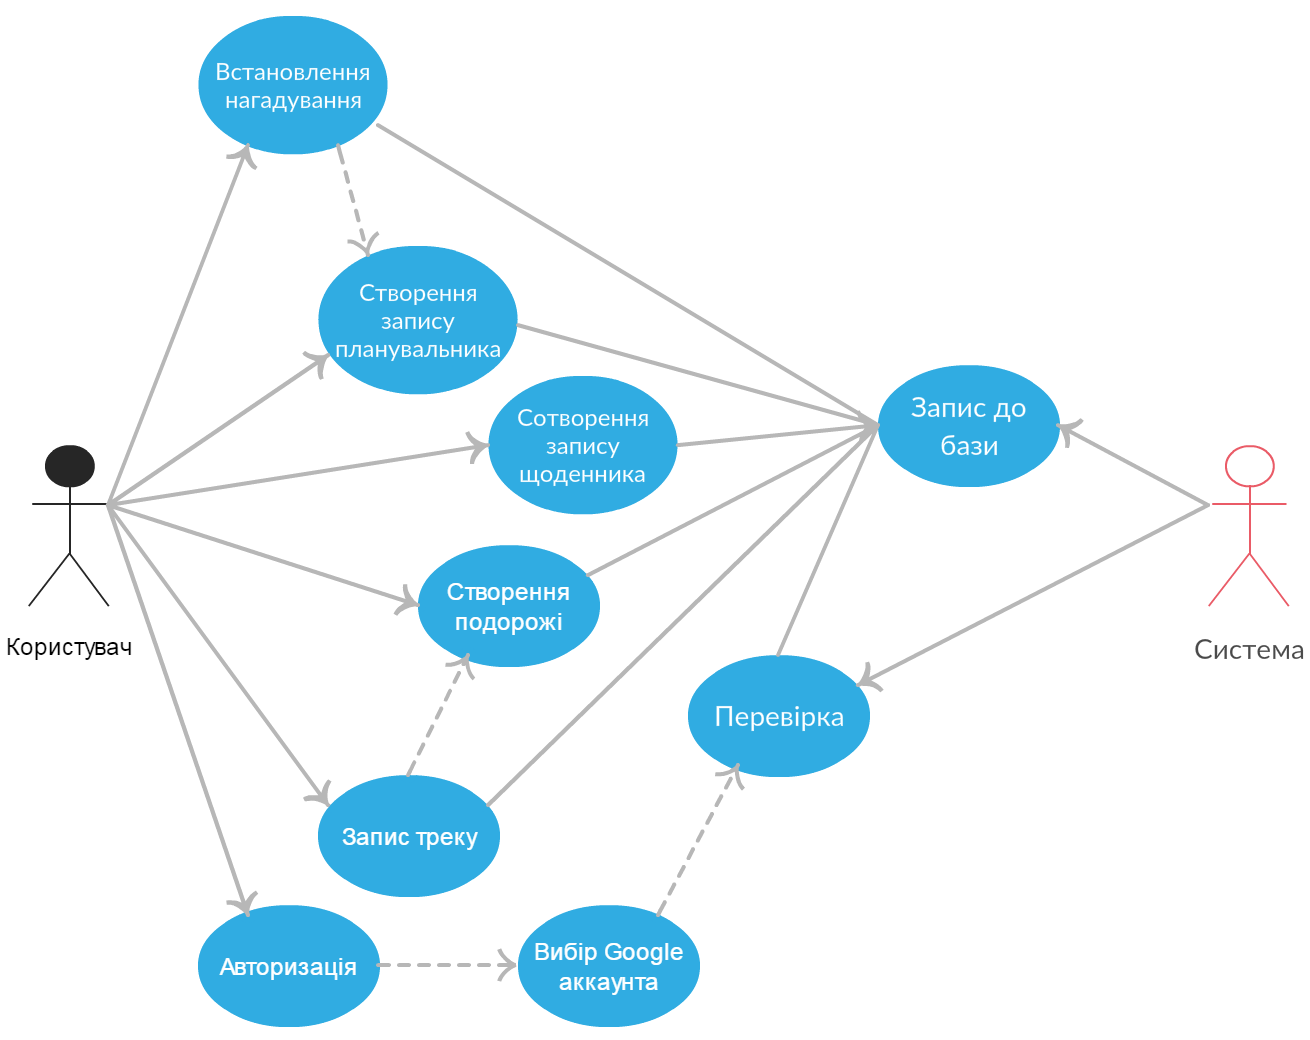
\includegraphics[width=1\textwidth]{diagram_usecase}
	\caption{Механізм роботи з додатком у вигляді діаграми прецедентів}
	\label{diagram:1}
\end{figure}

% TODO \subsection{Формулювання та аналіз вимог за допомогою діаграми діяльності}

\end{document}